%===============================================================
%   Implementation Report
%===============================================================

\documentclass[parskip=full]{scrartcl}

\usepackage{enumerate}
\usepackage[shortlabels]{enumitem}
\usepackage[utf8]{inputenc} % use utf8 file encoding for TeX sources
\usepackage[T1]{fontenc} % avoid garbled Unicode text in pdf
\usepackage{hyperref} % detailed hyperlink/pdf configuration
\usepackage{csquotes} % provides \enquote{} macro for "quotes"
\usepackage{graphicx} % embed graphics
\usepackage[toc]{glossaries}

% definitions
\newcommand{\pseProjectName}{An Interactive End-To-End Machine Learning Platform}
\newcommand{\pseTitle}{\pseProjectName}
\newcommand{\pseDocTitle}{Implementation Report}

\hypersetup{ % ‘texdoc hyperref‘ for options
pdftitle={\pseDocTitle}}
\title{%
    \pseTitle \\
    \large \pseDocTitle
    \date{\today}
}
\makenoidxglossaries
\loadglsentries{glossary}
\begin{document}

\begin{titlepage}
    \maketitle
    \begin{center}
        \begin{tabular}{ r l }
            Requirements Specification & \textbf{Murat Kurnaz}         \\
            Design                     & \textbf{Mustafa Enes Batur}   \\
            Implementation             & \textbf{Ömer Erdinç Yağmurlu} \\
            QA / Testing               & \textbf{Tarek Gaddour}        \\
            Final                      & \textbf{Atalay Donat}         \\
        \end{tabular}
    \end{center}
\end{titlepage}

\tableofcontents

\section{Tools}
\subsection{VS Code}
Code Editor
\subsection{PlantUML}
Charting software
\subsection{MikTEX}
Latex compiler and package manager
\subsection{npm}
node package manager
\subsection{create-react-app}
an intuitive command line scaffolding application easing the development of react applications

\emph{TBD, ADD MORE STUFF HERE, PYTHON ETC}
\newpage
\section{Challenges}
\subsection{Client}
\subsubsection{Testing Clients}
The front-end is written in React and is composed of presentational components (components), stateful components (containers) and hooks. In separating presentational and stateful components from one another we wanted to ease testing. Although testing presentational components took place without a problem using Jest.js snapshots, render tests and some simple consistency tests, stateful containers were harder to test, since they required extensive mocking of React's hook and lifecycle events.

\subsubsection{Sensor Data Collection}
\paragraph{Browser Inconsistencies} \

\textit{from https://github.com/PSE-TECO-2020-TEAM1/client/issues/5\#issuecomment-817308653}

There are two main APIs on sensor access in browsers right now, namely the Sensors API, which is incorporated into the web standard and supported by 71.03\% of all users worldwide.

On the other hand there is the legacy DeviceMotionEvent API, which was an experimental technology designed before the aforementioned Sensors API was drafted. It is supported by 94.97\% of users worldwide (albeit with handicaps).

In this application, we are using the new standard Sensors API, which is only supported by Chrome and Chromium based browsers like Edge, Brave etc. for now. Apple refuses to implement the new API citing privacy concerns, there is no information on why Firefox doesn't implement it. Since on Apple platforms all browsers from all vendors use the Safari WebView, this new API doesn't work at all on Apple devices.

The DeviceMotionEvent API is unfortunately not suitable for use at all. All three different major browsers (Chrome, Safari and Firefox) have a different understanding of what coordinates they return and have no documentation of which units they return the data in.

We've tried to use a polyfill with the branch sensors-polyfill, but were getting totally different results with different browsers (and with firefox totally broken results. Because of this reason we've decided not to support Apple users at all.

\paragraph{Magnetometer} \
Originally we wanted to support Magnetometer sensor too, since it was (supposedly) supported by the browsers we were targeting (on caniuse.com).
\begin{center}
\end{center}

\begin{figure}[ht]
    \centering
    \fbox{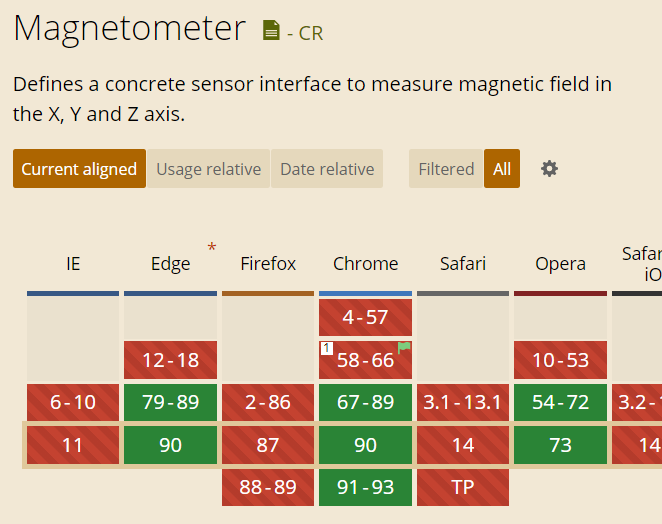
\includegraphics[width=\textwidth]{images/magneto1.png}}
    \caption{caniuse.com - Magnetometer}
\end{figure}



After implementing the sensor, however, we've noticed how no matter what we've tried, we weren't getting any data, and after more investigations we've discovered that the 'Magnetometer Sensor' and the 'Magnetometer Sensor API' are two different entities separate from each other, and dropped support for magnetometers.

\begin{figure}[ht]
    \centering
    \fbox{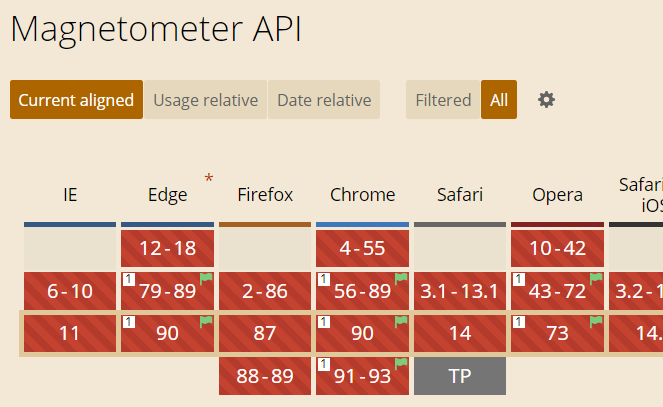
\includegraphics[width=\textwidth]{images/magneto2.png}}
    \caption{caniuse.com - Magnetometer API}
\end{figure}
\newpage
\subsection{Workspace Management}
\paragraph{Making a Consistent Server and Covering Failure Cases}
As the workspace management handles storage of user data, it acts as a bridge between the client and the model management. Thus the validity of these data is a very crucial part of the work. Although the client prevents most of the invalid requests, such invalid requests could be handcrafted and sent to the server or the client itself could possibly generate an invalid data by an error so each request needed to be validated. Finding the error cases and handling them generated a lot of work, because finding the not so obvious error cases needed a general analysis of the action caused by the request on the server and possibly on the model management.
\paragraph{Performance-Space Trade-Off Decisions}
Swaying from the initial design is in most cases undesirable and comes with a cost. However as the implementation phase progressed, it came to light that the initial design fell short on some aspects regarding the functionality (see \ref{changes}). The app is designed to be scalable so when introducing new changes to the codebase we had to take performance related issues into consideration and it slowed down the progress when the changes had conflicting aspects regarding performance and space.
\subsection{Model Management}
This was a very challenging part of the project for us, since we had no 
experience with the libraries that we use (namely scikit-learn) as well
as the programming language Python and the machine learning pipeline. Our first
attempt showed that our design for the service was not appropriate for the requirements
so we had to iterate twice, which included writing the whole service from
stratch.

\subsubsection{Understanding Machine Learning Pipeline}
During the design phase, we had tried to get a grasp of the machine learning
process that we were going to implement but we had no real experience with it.
This resulted in a very abstract design since we were unsure how different
mechanisms interacted with each other. As we experimented with the frameworks,
a series of new requirements came into play. This included changes in other
components of the system that Model Management depended on like the front-end
clients. As a result, we had to constantly communicate with each
other, synchronize our works and give feedback to each other. With time, our
better understanding of the machine learning process made things easier and
allowed us to solve problems quickly.

\subsubsection{Caching Mechanism and MongoDB Document Size Restrictions}
The first issue that we have faced was the caching mechanism for the processed
data which helped the training with avoiding repetitive calculations when
possible. Our first naive approach was to store everything in an array. It
became quickly apparent that saving the data this way complicated the code
immensely and was very error prone. The solution was to store serialized
DataFrame objects as a document in the database. During the testing we realized
that MongoDB did not allow for documents larger than 16 MB in size. Another
framework (GridFS) that wrapped MongoDB allowed us to solve this problem and
store files without any size restrictions.

\subsubsection{Multiprocessing and Serving Many Clients in Parallel}
The biggest challenge of the Model Management service was allowing multiple
training or prediction processes take place on the server in parallel. Because
of the computing intensive nature of the machine learning processes, it was
not feasiable to run the training or prediction on the same process that handled
the client requests which would greatly reduce the server responsiveness.
After a through research on possible solutions, we have decided that the 
best solution was to spawn new processes for each computing intensive task (i.e.
training/prediction), since we discovered that multithreading does not work as
expected in programming languages that depend on an interpreter. The hardest part
was to synchronize the processes and handle the interprocess communication. The solution for data transfer between
the server and the child processes was using Unix Pipes and the synchronization
problem was solved by using counting semaphores.
\subsection{Auth}
No notable challenges.
\newpage
\section{Statistics}
\subsection{client}
\begin{tabular}{ c|c } 
    Lines of code & TBD \\ 
    Test coverage & TBD \\ 
    Number of commits & RBD \\ 
\end{tabular}

\subsection{workspace-management}
\subsection{model-management}
\subsection{auth-management}
\subsection{Total}
\newpage
\section{Changes from Design}
\subsection{Authentication}
No notable changes.

\newpage
\subsection{client}
\subsubsection{Single Codebase}
In the design document, we'd envisioned two different codebases for the different edge (mobile) and management (desktop) clients. During development, however, it has become obvious that a single codebase with client side routing and bundle separation using tree shaking was more suitable for our application. We are bundling both applications in a single router, and there is no clear separation between each client. During development, special care was given to reduce cross dependencies between both parts to a minimum in order to reduce the bundle size for edge devices.

\subsubsection{/lib folder}
Originally, there were only two auxiliary classes in the whole client (MobileAPI and DesktopAPI), while everything else was a React component. During development, we made use of custom react hooks (/lib/hooks) to refactor common stateful logic into reusable parts. Apart from hooks, sensor data collection needed it's own abstraction over the clunky Web API implementation, which we've placed in /lib/sensors.

\subsubsection{API endpoints}
In order to accomodate changes in the backend, both the Mobile- and DesktopAPI have undergone major changes in the interfaces they implement.

\subsubsection{Component Library}
In the design document, we'd specified Material-UI as the component library that we were going to use. During development we've found it too clunky, heavy and hard to develop with and replaced it with the Evergreen Component Library from segment.io. This component library also comes with it's own opinionated 'CSS-in-JS' styling library, through which we were able to style the application with a rapid pace.

\subsubsection{ModelOptions Component}
This component faced the most changes during implementation. We'd decided to distribute some model creation options to the sensor-components themselves instead of using the same set of parameters for each component. This had it's implications on the client and it had to be updated accordingly.

\begin{figure}[ht]
    \centering
    \fbox{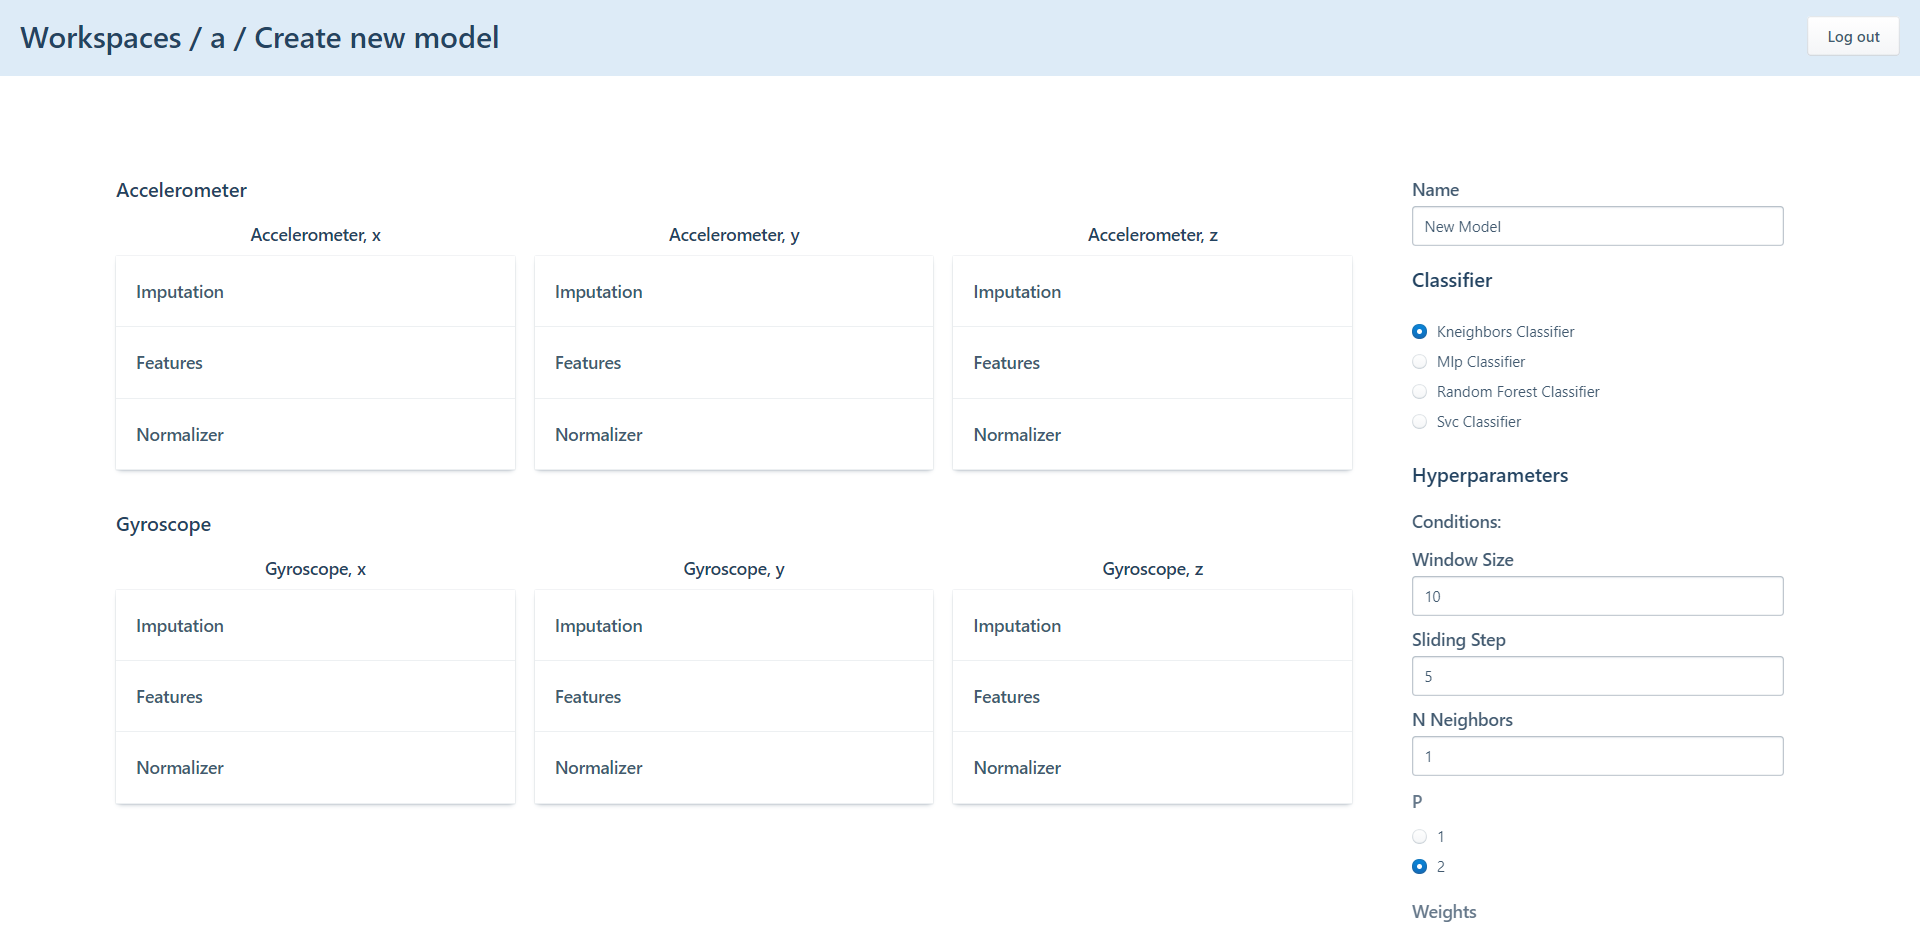
\includegraphics[width=\textwidth]{images/v-modelpng.png}}
    \caption{New ModelOptions}
\end{figure}

\begin{figure}
    \centering
    \fbox{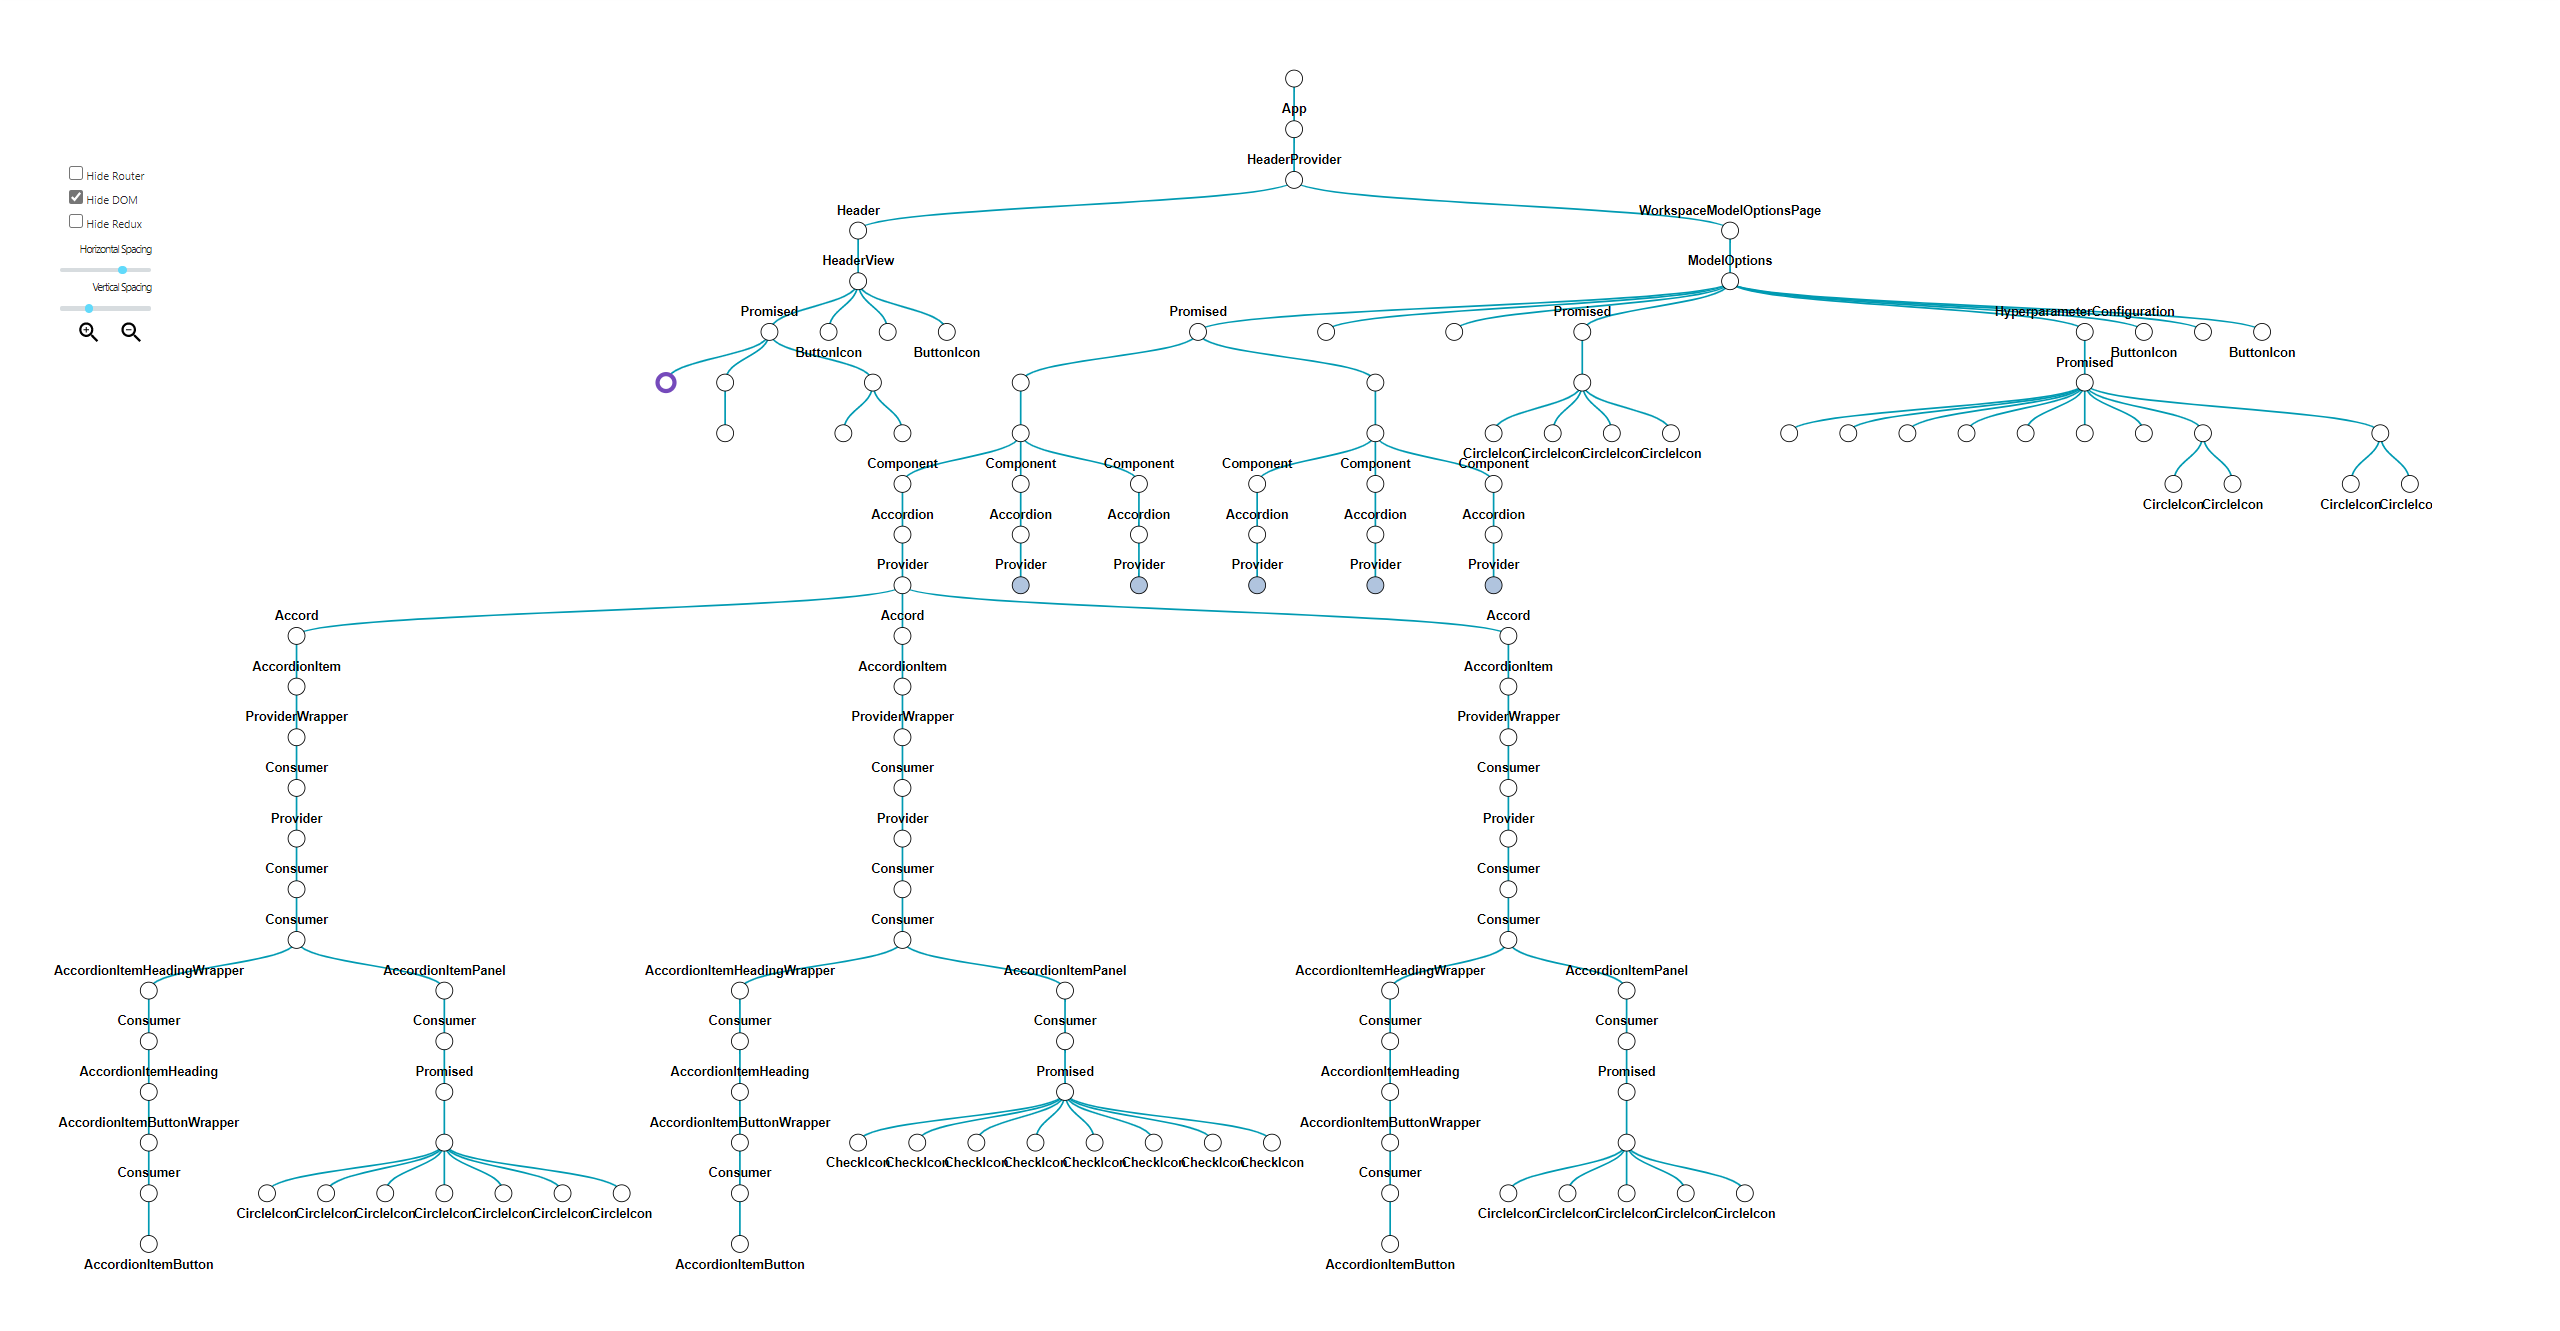
\includegraphics[height=1.2\textheight]{images/ch-model.png}}
    \caption{New ModelOptions Component Graph}
\end{figure}
\newpage
\subsection{Workspace-Management}
\subsubsection{Label}
Label isn't saved as an embedded document anymore. To achieve the same functionality label now keeps the workspaceId of the workspace it belongs to and the number of samples it is the label of.
\subsubsection{Data Point}
ObjectId is now omitted as it is not used and causes disarray in the corresponding responses.
\subsubsection{Sensor Data Point}
ObjectId is omitted here as well on the same grounds. In addition name of the sensor is also added to schema to simplify communication with the client.
\subsubsection{Sample}
Sample does not embed the label data anymore, instead it saves the id of the label. Implementation of setTimeFrames method is also delegated to the workspaceController.
\subsubsection{Workspace}
\paragraph{SubmissionId} SubmissionId is not saved as a simple string anymore, instead it has its own interface with the field hash as string. This change was done to provide flexibility for possible future use cases, such as making submissionId expire after a while etc.
\paragraph{Further Additions} Workspace now holds lastModifiedDate to enable model management to cache the machine learning pipeline, sample- and labelIds to speed up database queries/checks.
\subsubsection{Routes}
\paragraph{General Changes} Added new bad request responses that explains the error user is getting.
\paragraph{GET /api/sensors} Removed as it didn't provide any utility other methods didn't cover.
\paragraph{GET /api/workspaces/{workspaceId}/samples} Query parameters are changed to showDataPoints and onlyDate to be more intuitive.
\paragraph{GET /api/workspaces/{workspaceId}/samples/{sampleId}} Response now also includes the timeframes of the sample.
\paragraph{PUT /api/workspaces/{workspaceId}/samples/{sampleId}/relabel} labelName is now passed in the query instead of labelId.
\paragraph{GET /api/workspaces/{workspaceId}/labels} Response body now also includes the sample count of the label.
\paragraph{POST /api/workspaces/{workspaceId}/labels/create} labelName is now passed in the body instead of the query.
\paragraph{PUT /api/workspaces/{workspaceId}/labels/{labelId}/rename} labelName is now passed in the body instead of the query.
\paragraph{PUT /api/workspaces/{workspaceId}/labels/{labelId}/describe} description is now passed in the body instead of the query.
\paragraph{GET /api/workspaces/{workspaceId}/submissionId} This route has been changed to GET /api/workspaces/{workspaceId}/generateSubmissionId to make its function clear.
\paragraph{GET /api/submissionConfig} Label objects now include their labelId in the response body.
\paragraph{POST /api/submitSample} submissionId is now passed in the request body.

\newpage
\subsection{Model Management}
As described in the challenges section, we had to redesign this service. The main
reason is the multiprocessing needs of the application that was unforeseeable for
us during the design phase. The complete changelog requires a completely new design
document but the following are the most important changes.

\subsubsection{Router}
\begin{itemize}
    \item 
    Split the Router class into two classes, CommonRoutes and WorkspaceRoutes.
    \newline
    \textbf{Reason:} API endpoints that need authentication are all under
    a specific workspace, so the split made it easier to handle the authentication
    of requests. We use an authentication middleware for all workspace routes. 
    \item
    Removed generatePredictionId method
    \newline
    \textbf{Reason:} We delegate this responsibility to the MongoDB client that
    generates a new ID for each document that is inserted into the database.
    \item
    Removed the trainers and predictors fields
    \newline
    \textbf{Reason:} Trainers map was planned to be used to track the progress.
    Since each trainer starts in a new process, this was not possible and we used
    the database for progress tracking instead. Predictors are in a new class
    PredictionManager described below.
\end{itemize}

\subsubsection{Request and Response Classes}
\begin{itemize}
    \item
    Renamed the data classes.
    \newline
    \textbf{Reason:} The classes now represent the actual content instead of the name
    of the API endpoint (i.e. TrainReq -> TrainingConfig)
    \item
    Seperate (sometimes duplicate) classes for domain models and API models
    \newline
    \textbf{Reason:} The first iteration of the service showed us that using the
    same models for both internal logic and API endpoints are problematic because
    of the possible changes to the endpoints. By seperating the classes, we had
    the flexibility to change endpoints/parameters without affecting the logic code,
    since the API models are converted to domain models.
    \item
    Added data validation for endpoints 
    \newline
    \textbf{Reason:} During the design, the data validation was missing. We have
    added the data validation for models with comprehensible error messages that
    frontend shows the end users.
\end{itemize}

\subsubsection{Database}
\begin{itemize}
    \item
    Added wrapper classes for database queries
    \newline
    \textbf{Reason:} At first we were calling the functions of PyMongo directly in
    the application code. We thought this was not a good idea as it was not possible
    to use a different database. With that in mind, we implemented several wrapper
    classes which implement database queries.
\end{itemize}

\subsubsection{Database Models}
\begin{itemize}
    \item
    Added (de)serialization methods for database models
    \newline
    \textbf{Reason:} We save large data in the database in binary form. 
    (bytes type). To prevent errors during the deserialization because of the
    unknown type of the binary objects, we added methods that complete
    the type information for each binary document to database model classes.
\end{itemize}

\subsubsection{Training}
\begin{itemize}
    \item
    Training a model is handled by a new process
    \newline
    \textbf{Reason:} The training of a model takes a notable amount of time,
    especially if there are a lot of samples. If the main process were to train
    the model, any requests during the training could only be handled after the
    training is finished. This was a terrible idea, so a new process is created
    to handle the training and the main thread is then able to handle other
    requests during the training.

    \item
    Added DataSetManager and TrainingManager classes
    \newline
    \textbf{Reason:} The Trainer class which we initially designed was a typical
    God object in which the training pipeline, all the training algorithms and
    the database queries are implemented. With seperation of concerns in mind, we
    decided to split this Trainer class in three classes: DataSetManager handles 
    the database queries, the Trainer class has all the algorithms implemented and
    the TrainingManager handles the training pipeline.
\end{itemize}

\subsubsection{Prediction}
\begin{itemize}
    \item
    Prediction is handled by a new process
    \newline
    \textbf{Reason:} This has the same motivation with handling the training with a
    new process: Being able to handle other requests while a prediction is under way.

    \item
    Added DataSetManager and PredictionManager classes
    \newline
    \textbf{Reason:} This also has the same reasoning with the training: The Predictor
    class we had was a typical God object. The DataSetManager handles the database
    queries, the Predictor class implements all the algorithms and the PredictionManager
    handles the prediction pipeline.
\end{itemize}
\newpage
\newpage
\section{Functional Requirements Coverage}
\subsection{Mandatory Requirements}
\begin{center}
    \resizebox{\textwidth}{!}{\begin{tabular}{c||c|c|c} 
        Number & Requirement Name & Implemented? & Notes \\ [0.5ex]
        \hline
        F010 & Show a welcome page with a login panel when the website is accessed & YES &  \\
        F020 & Show registration panel when clicked on register in the welcome page & YES &  \\
        F030 & Show a workspaces overview where the available workspaces are listed after logged in & YES &  \\
        F040 & Allow creating workspaces with the given name, sensors to be used and their sampling rate & YES &  \\
        F050 & List the available sensors (accelerometer and gyroscope) for the recordings on the workspace creation window & YES &  \\
        F060 & Show the workspace panel when a workspace is selected & YES &  \\
        F070 & Allow renaming workspaces on the workspace panel by double clicking on the workspace name & YES &  \\
        F080 & List labels with their sample count on the labels overview window  & YES &  \\
        F090 & Allow creating labels for the actions to be recorded in the workspace  & YES &  \\
        F100 & Allow renaming labels on the labels overview & YES &  \\
        F110 & Allow deleting labels which in turn deletes the data samples with the selected label & YES &  \\
        F120 & Display a link to be used for recording data to the workspace when collect data is clicked & YES &  \\
        F130 & Display a button to copy the link to the clipboard & YES &  \\
        F140 & Display QR code with the same link in the previous function embedded to be used for recording data & YES &  \\
        F150 & Display the collected data samples chronologically on the workspace panel & YES &  \\
        F160 & Visualize the selected data sample as a graph when the data sample is clicked on the workspace panel & YES &  \\
        F170 & Allow changing the graph type & NO & (0) \\
        F180 & Display the metadata of the selected data sample (identifier of the recording device and recording date/time) & YES &  \\
        F190 & Allow setting the start/end time of the labeled actions on the graph view of the selected data sample & YES &  \\
        F200 & Allow relabeling the selected data sample & YES &  \\
        F210 & Allow deletion of the selected data sample & YES &  \\
        F220 & Allow selecting data imputation options on the workspace panel & PARTIALLY & (1) \\
        F230 & Allow selecting feature extration options on the workspace panel & YES &  \\
        F240 & Allow selecting normalization options on the workspace panel& YES &  \\
        F250 & Allow selecting machine learning model on the workspace panel with hyperparameters & YES &  \\
        F260 & Request training of the model according to the selected options and automatically deploy it & YES &  \\
        F270 & List trained and deployed models on the models overview & YES &  \\
        F280 & Show the overview of the selected model when clicked on a model on the models overview & YES &  \\
        F281 & Display the used parameters of the selected model & YES &  \\
        F282 & Display the performance metrics of the selected model & PARTIALLY & (2) \\
        F290 & Display a mini QR code symbol for each model on the models overview & YES &  \\
        F300 & Display a link to use the deployed model on mobile devices when the mini QR code symbol is clicked & YES &  \\
        F310 & Display a button to copy the link to the clipboard & YES &  \\
        F320 & Display QR code with the same link in the previous function embedded to be used for classifying data & YES &  \\
        F330 & Display a logout button on all pages Mobile Web Client & YES &  \\
        F340 & Show a list of available labels that will label the recorded data when the data collection is initiated & YES &  \\
        F350 & Show an error if not all the required sensors are available in the device & YES &  \\
        F360 & Allow configuring the countdown duration until the recording starts & YES &  \\
        F370 & Allow configuring the recording duration & YES &  \\
        F380 & Show a button to initiate the recording & YES &  \\
        F390 & Show a countdown page with the current configuration on display (label, sensors used and their sampling rates) & YES &  \\
        F400 & Display the sensor data in real-time as curves for each sensor on a single graph & YES &  \\
        F410 & Show a recording completed page when the recording duration times out  & YES &  \\
        F420 & Allow discarding the last recording  & YES &  \\
        F430 & Allow another recording with the same configuration  & YES &  \\
        F440 & Allow editing configurations for the next recording  & YES &  \\
        F450 & Show a page for classification when the link of a model is opened & YES &  \\
        F460 & Start listening to the sensor data of the mobile device right after the page is loaded & YES &  \\
        F470 & Display the sensor data in real-time as curves for each sensor on a single graph  & YES &  \\
        F480 & Display the classified actions on the webpage in real time  & YES &  \\
        F490 & Allow stopping the recording & YES &  \\
        F500 & Display the classified actions as a chronological list when the recording is stopped & YES &  \\
        F510 & Allow restarting the recording 5.1.2 Server API & YES &  \\
        F520 & Serve authentication services  & YES &  \\
        F530 & Handle workspace information  & YES &  \\
        F540 & Handle workspace data set.  & YES &  \\
        F550 & Handle label information for a workspace  & YES &  \\
        F560 & Store data coming from a mobile client  & YES &  \\
        F570 & Initiate the configured model training  & YES &  \\
        F580 & Handle model information for the workspace & YES &  \\
        [1ex] 
   \end{tabular}}
\end{center}
(0): one graph type only

(1): Not all imputers implemented

(2): Not all metrics implemented

\subsection{Optional Requirements}
\begin{center}
    \resizebox{\textwidth}{!}{\begin{tabular}{c||c|c|c} 
        Number & Requirement Name & Implemented? \\ [0.5ex]
        \hline
        F590 & Serve a "Stay Signed In" functionality on the desktop web client & NO \\
        F600 & Add CAPTCHA to login after 5 consecutive failed login attempts & NO \\
        F610 & Show a sign if a data collecting device is currently active & NO \\
        F620 & Allow listing samples by label on the workspace panel & NO \\
        F630 & Allow adding descriptions to the labels to assist data collection & YES \\
        F640 & Give the user non-visual feedback if an action is identified & NO \\
        F650 & Set a sound feedback to play when an action is identified & NO \\
        F660 & Serve a list of languages for the user interface & NO \\
        F670 & Support magnetometer sensor & NO \\
        F680 & Serve a "Forgot password" option that allows users to recover credentials & NO \\
        [1ex] 
   \end{tabular}}
\end{center}
\newpage
\section{Planned Schedule}
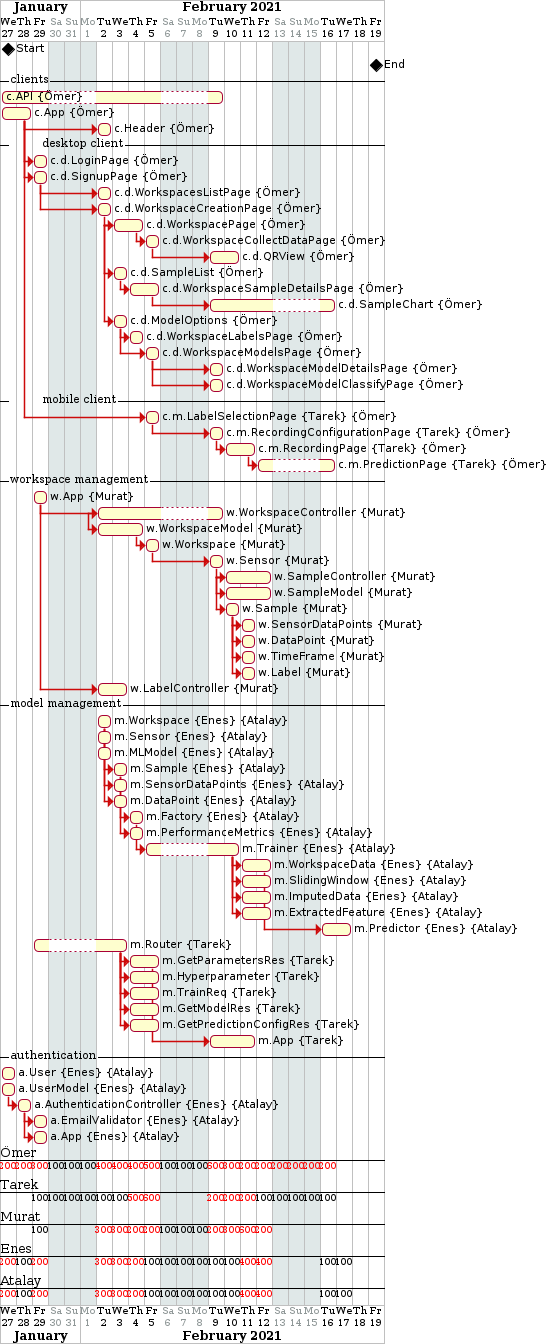
\includegraphics{images/gantt_orig.png}
\newpage
\section{Actual Schedule}
\centering
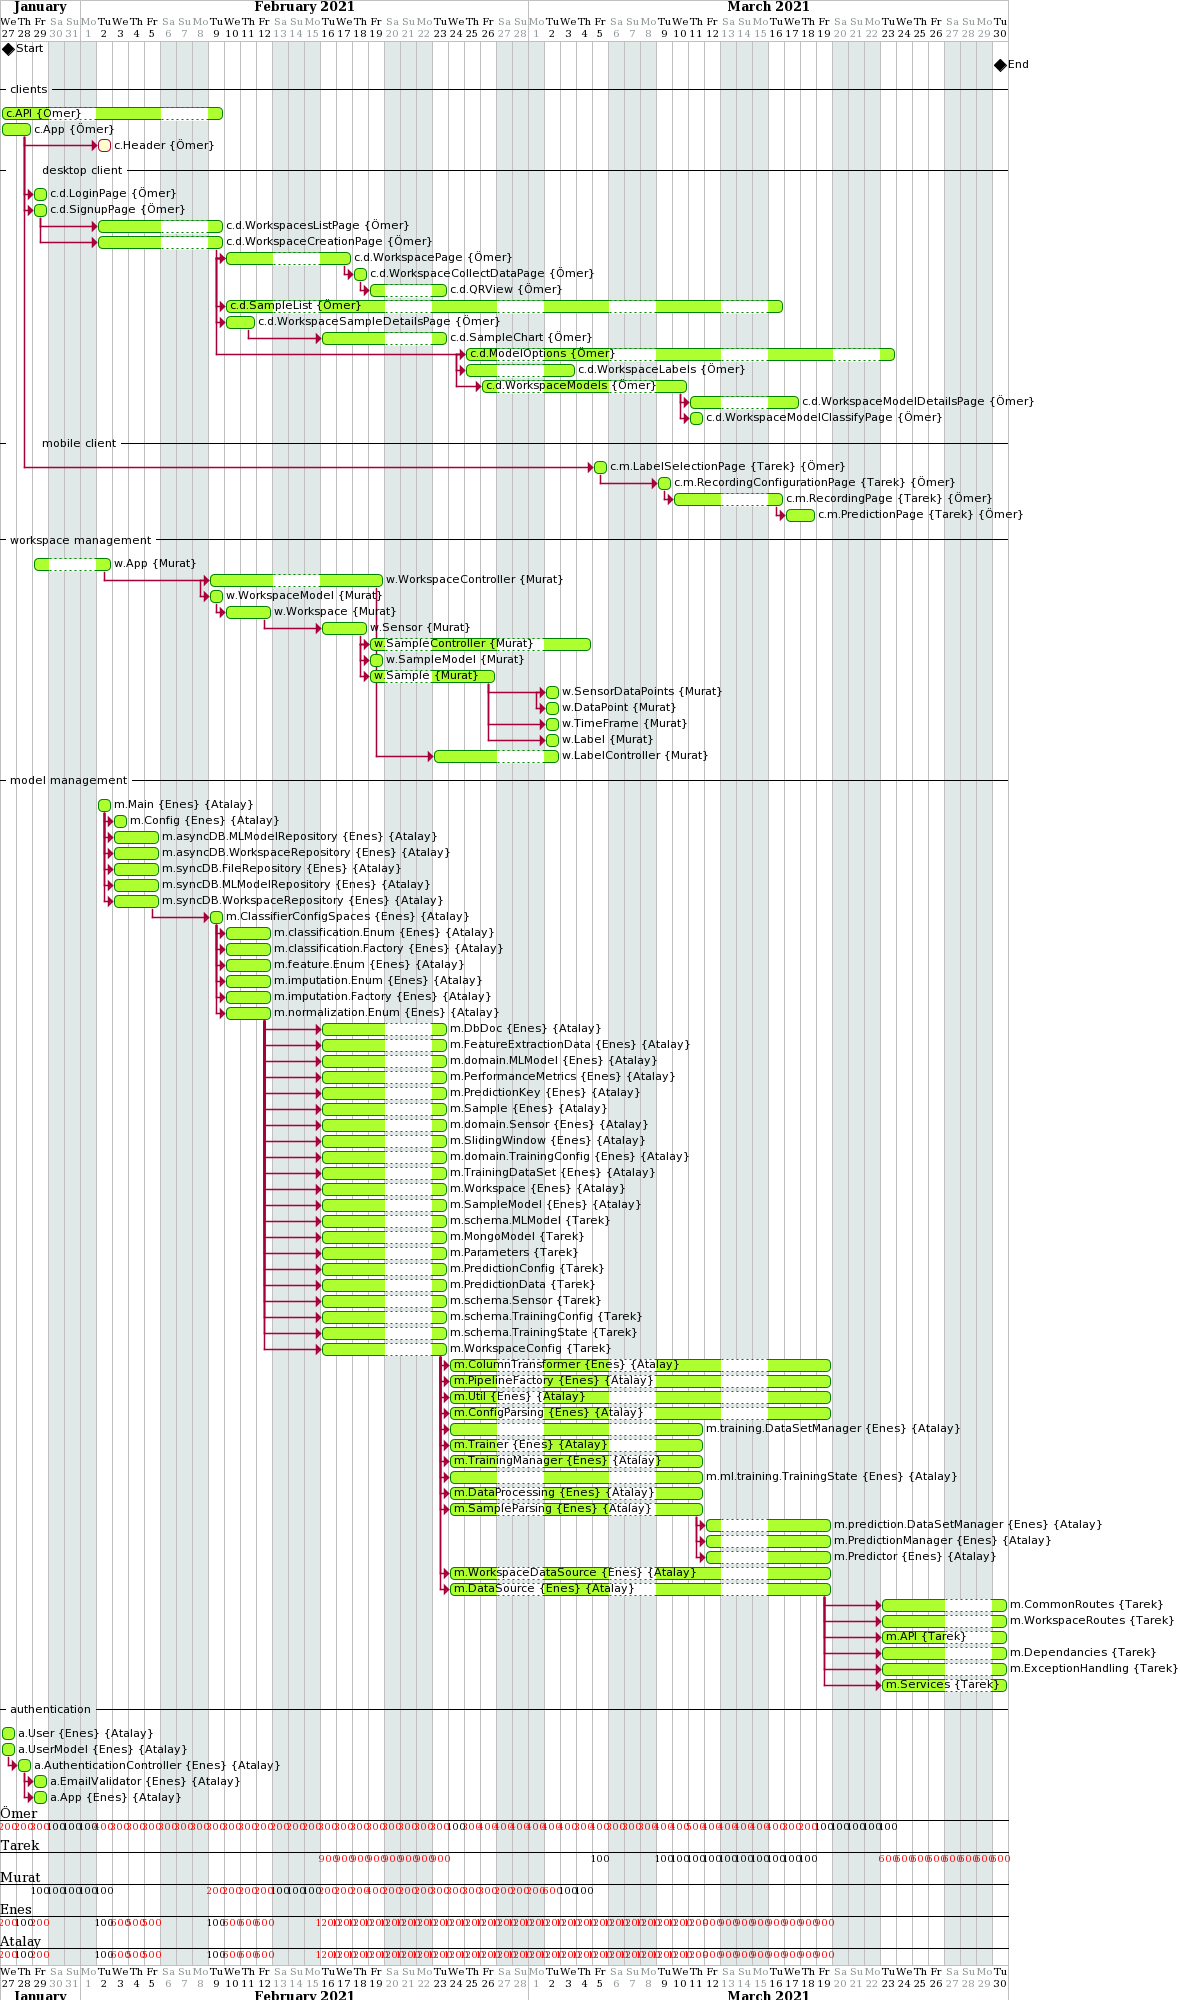
\includegraphics[height=0.9\textheight]{images/gantt.png}
\newpage
% \section{Unit Tests}
TBD
% \newpage
% \include{sections/integration-tests}
% \newpage

\printnoidxglossary

% END DOCUMENT
\end{document}
